\section*{Problem 7}
The goal of this problem is to visualise how similar different animals at a zoo are by projecting the given data from $\mathbb{R}^{16}$ to $\mathbb{R}^{2}$ using three different embeddings; PCA, MDS and Isomap. The data matrix $Y$ will be structured in the same way as in the lecture such that a column of $Y$ corresponds to a data point, thus is $Y \in R^{16 \times 101}$ as there are $101$ data points.

\subsection*{Preprocessing the data}
In order to enable the applications of the embeddings the data has to be preprocessed by first removing the columns 'type' and 'animal name' from the data set. These can later be used in the visualisation.

The remaining attributes are all boolean with values in $\{ 0,1 \}$ except the attribute 'legs' which takes values in $\{ 0, 2, 4, 6, 8 \}$. This attribute thus takes on values up to $8$ times the magnitude in comparison to the remaining attributes which results in the legs attribute to be seen as more important for the embeddings. For this reason the magnitude of 'legs' will be scaled down by $8$ times, causing it to instead take values in  $\{ 0, \frac{1}{4}, \frac{1}{2}, \frac{3}{4}, 1 \}$ giving it a similar magnitude to the remaining attributes.

\subsection*{Visualisation of data}
In order to project the data in 2D such that similar animals are projected close to one another the first two resulting latent variables from a method will be plotted against each other as they contain the most information about the data set as a result of the sorting of the singular values and eigenvalues in descending order.


\subsection*{PCA}
The implementation of PCA was solved in the following manner

\begin{algorithm}[H]
\SetAlgoLined
\KwInput{Data matrix $Y$}
\KwOutput{2-dimensional embedding $X$ }
\KwData{Zoo animals}
 Center the columns (data points) of the data matrix: $Y_c \gets \text{center}(Y)$

 Compute SVD of $Y_c$: $[U,\Sigma, V] \gets \text{SVD}(Y_c)$

 Select the first two columns of $U$: $W \gets [u_1, u_2]$

Compute embedding: $X \gets W^T Y_c$
 \caption{PCA method}
\end{algorithm}


The implementation was quite short using Numpy's Singular Value Decomposition function. The only concern that arised was the centring of the data matrix as it removes the boolean nature of the matrix. However I argue that this only translates the data points and does not remove the information of the attributes which renders the action viable.
\\

The following visualisation was achieved

\begin{figure}[H]
  \centering
  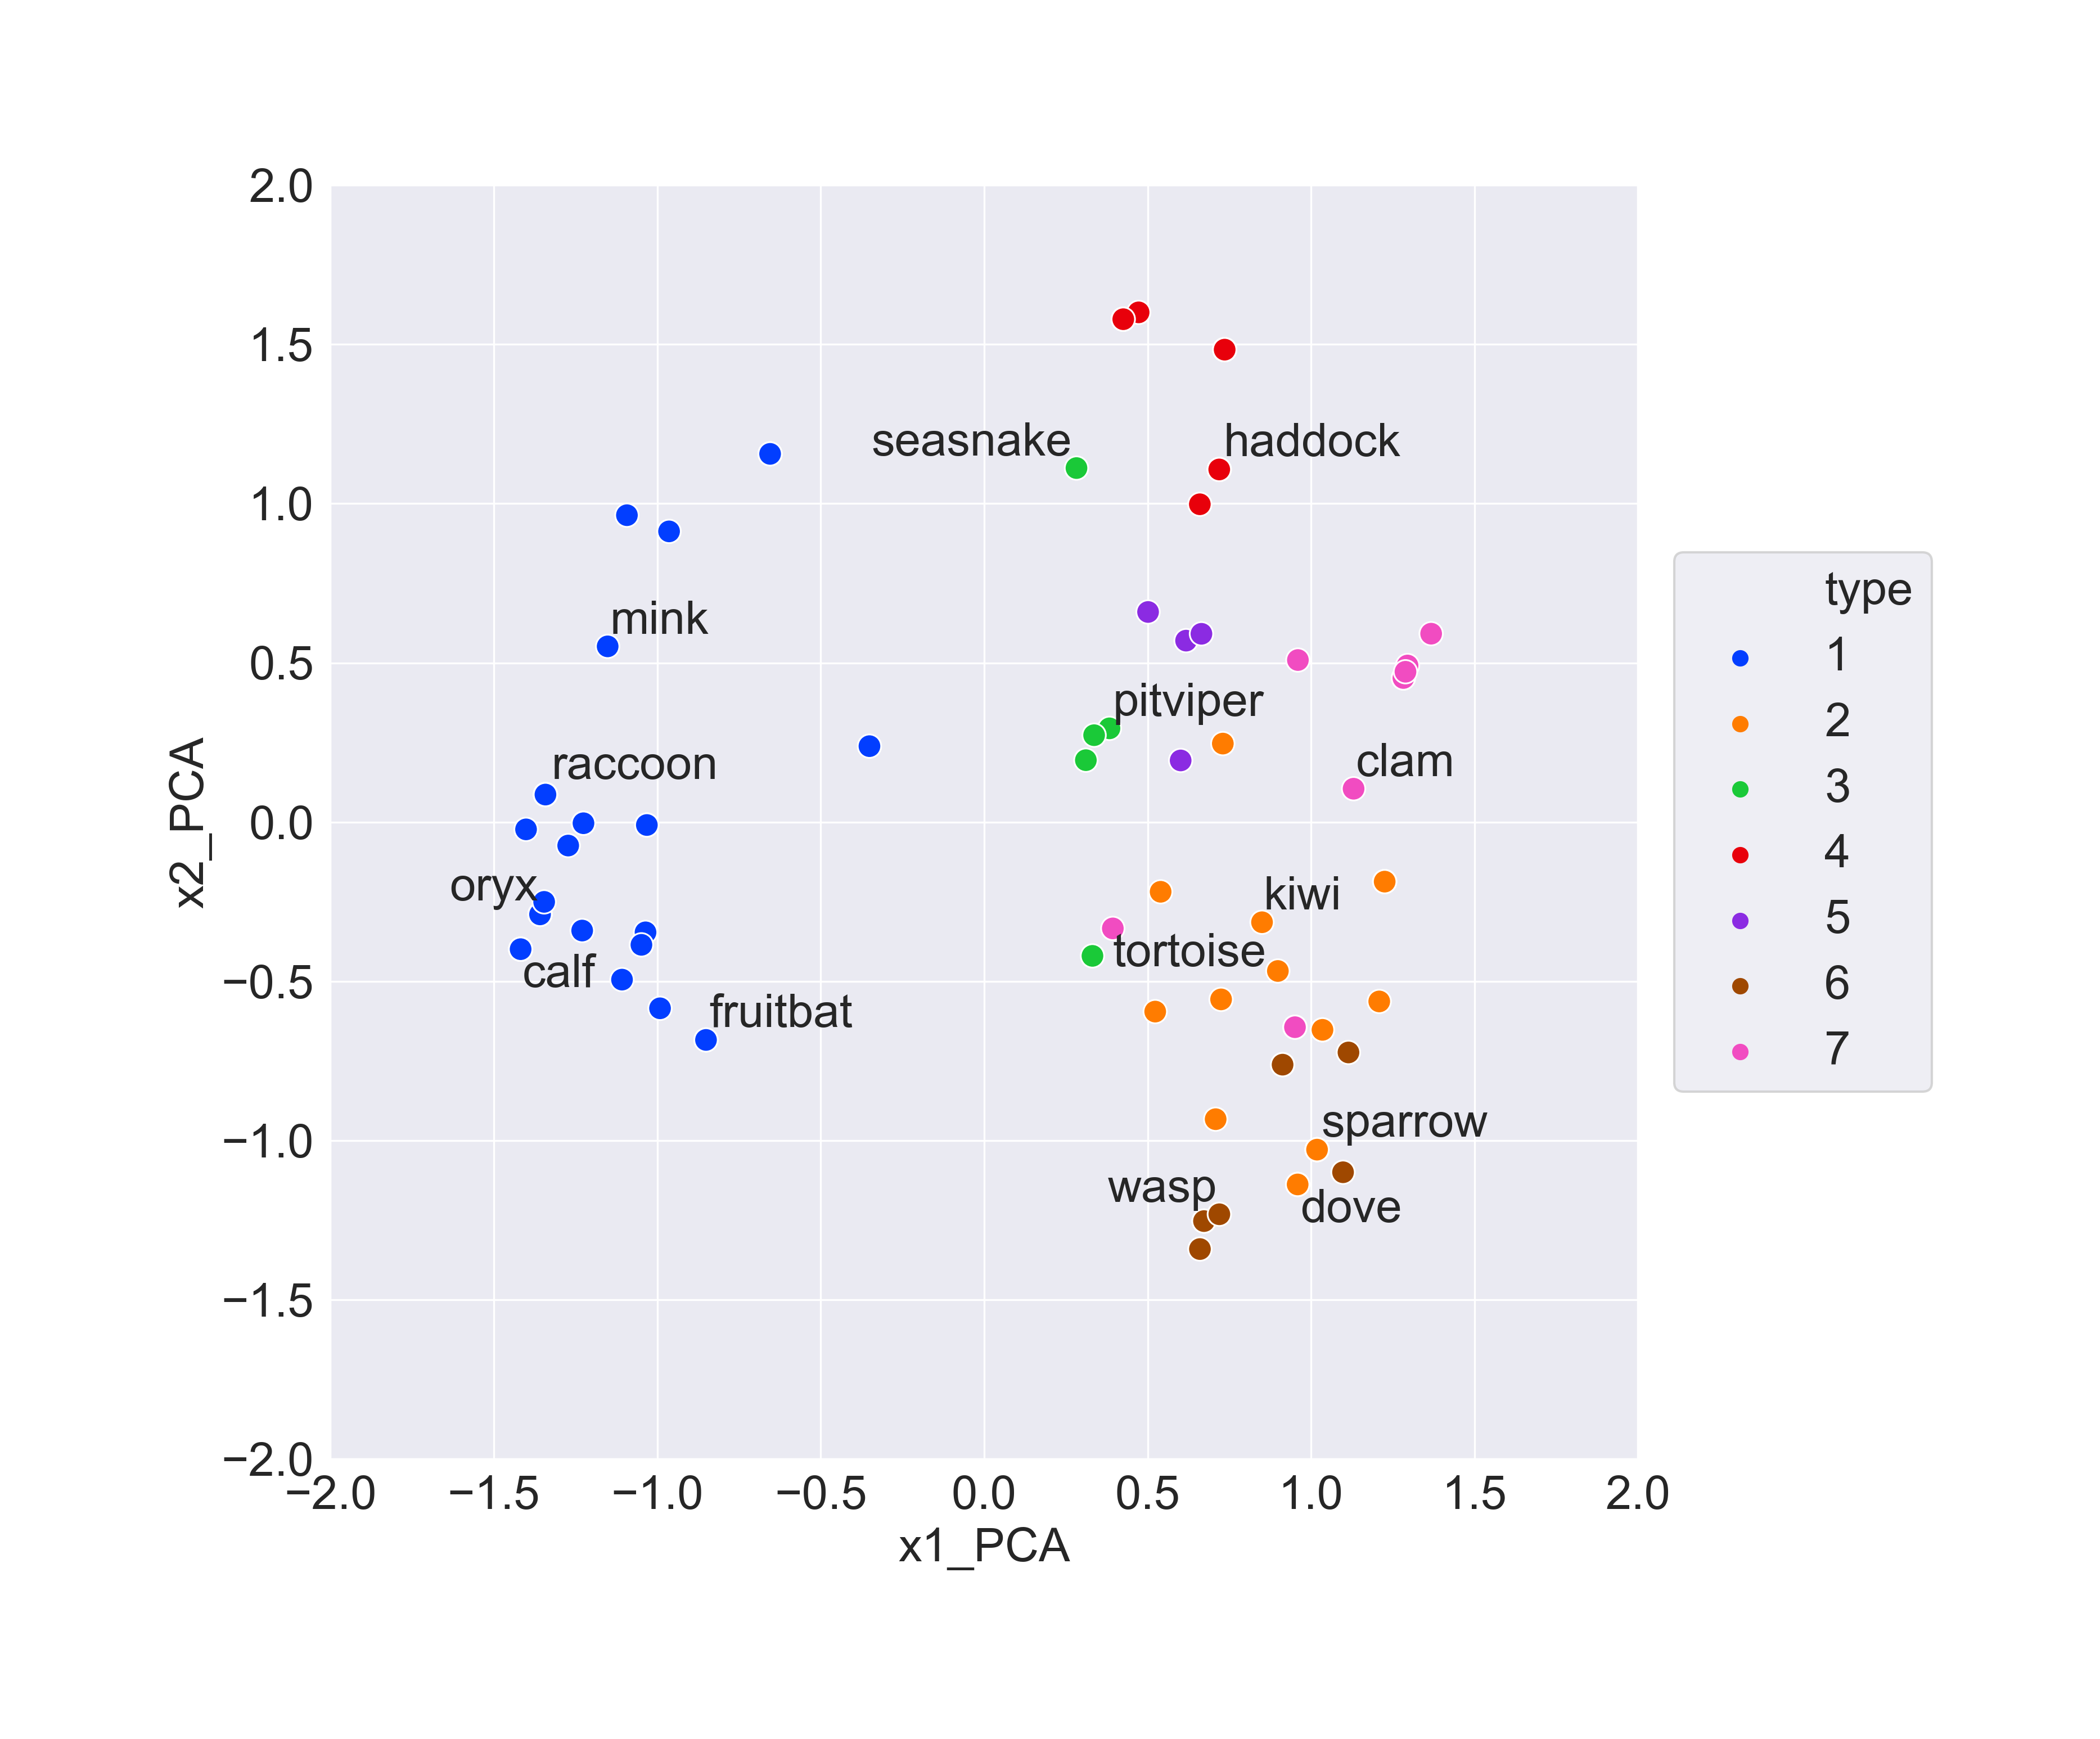
\includegraphics[width = 0.8\linewidth]{../Visualization_PCA.png}
  \caption{Visualisation PCA}
  \label{vis_PCA}
\end{figure}

where a few animals are annotated to give some intuition and understanding behind the placing of the different animals. It is apparent from the plot that there is a clear distinction between type $1$ and the remaining types $2-7$ whom are more mixed among each other.


\subsection*{MDS}
The implementation of MDS was solved in the following manner

\begin{algorithm}[H]
\SetAlgoLined
\KwInput{Data matrix $Y$}
\KwOutput{2-dimensional embedding $X$ }
\KwData{Zoo animals}
  Compute a distance matrix of the data: $D \gets \text{weighted\_distance} (Y) $

  Compute a similarity matrix from $D$: $S \gets \text{similarity\_matrix} (D) $

  Compute Eigen-decomposition of $S$: $[D,Q] \gets \text{Eig}(S)$

  Order $D$ in descending order of eigenvalues magnitude and $Q$ correspondingly

  Ensure elements of $D$ and $Q$ are real

  Compute embedding: $X \gets I_{2\times 101}D Q^T$

  \caption{MDS method}
\end{algorithm}


In the implementation of MDS it was proposed to infer the importance of different attributes by taking it into account when computing the pairwise distance. I solved this by replacing the pairwise distance $d(y_i, y_j)$ with $d_w(y_i, y_j)$ where

\begin{align*}
  & d(y_i, y_j) = \|y_i -y_j \|^2 = (y_i-y_j)^T(y_i-y_j)\\
  & d_w(y_i, y_j) = (y_i-y_j)^T W (y_i-y_j)
\end{align*}

 $y_i, y_j$ are two data points and $W = diag(w_1,w_2,..., w_k)$ where each $w_i$ is a weight for the corresponding attribute. If $w_i = 1, \forall i$ it is the same distance as before but if one weight, lets say $w_1 = 2$ attribute is twice as important as before since if that attribute differs between $y_i, y_j$, that distance is multiplied by $2$ now.

One concern that arose during the implementation of MDS was that the eigenvalues and eigenvectors had small complex components even though the matrix was symmetric. I believe that this was caused by the numerical imprecision of the computer and solved it by simply removing the complex components.

The following visualisation was achieved

\begin{figure}[H]
  \centering
  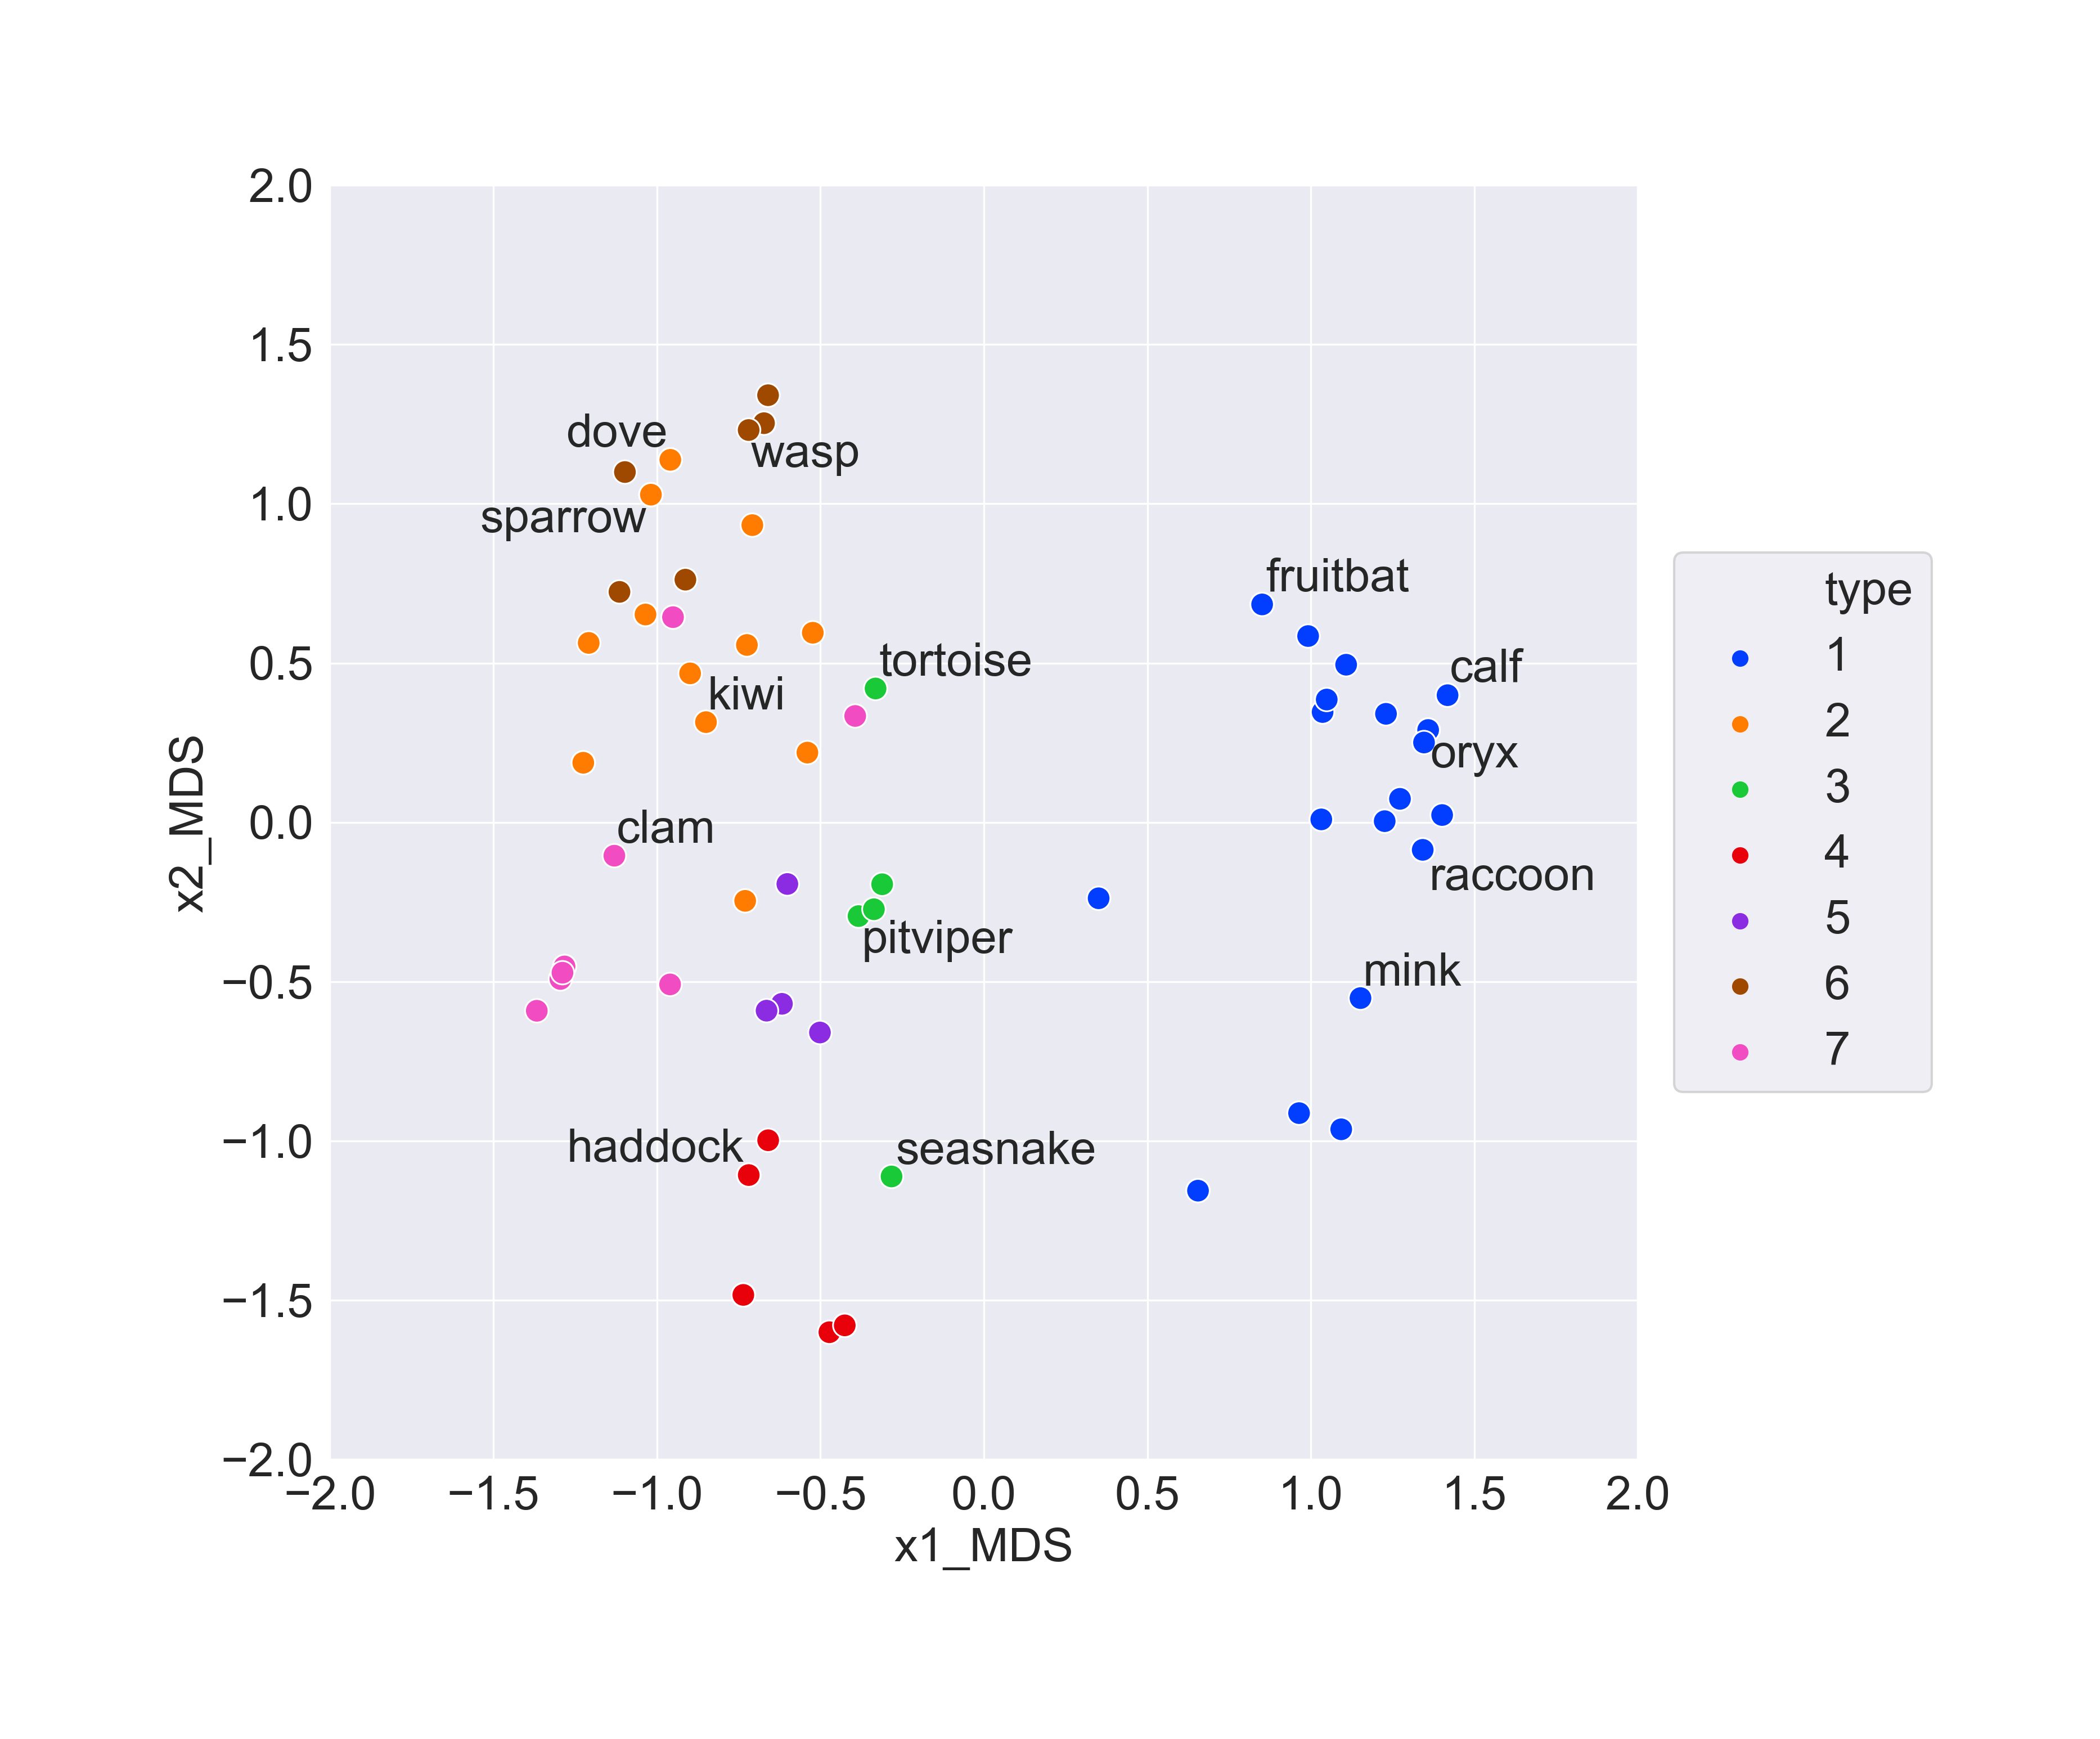
\includegraphics[width = 0.8\linewidth]{../Visualization_MDS_no_weights.png}
  \caption{Visualisation MDS, all weights equal to $1$}
  \label{vis_PCA}
\end{figure}

Here one can see that using all weights equal to $1$ yields a very similar result to the one of PCA only that the points are mirrored over both the y and x axis which I believe is a result of the eigenvalue algorithm of Numpy since one can change the sign of an eigenvector and it still fulfils the eigenvalue equation.
\begin{figure}[H]
  \centering
  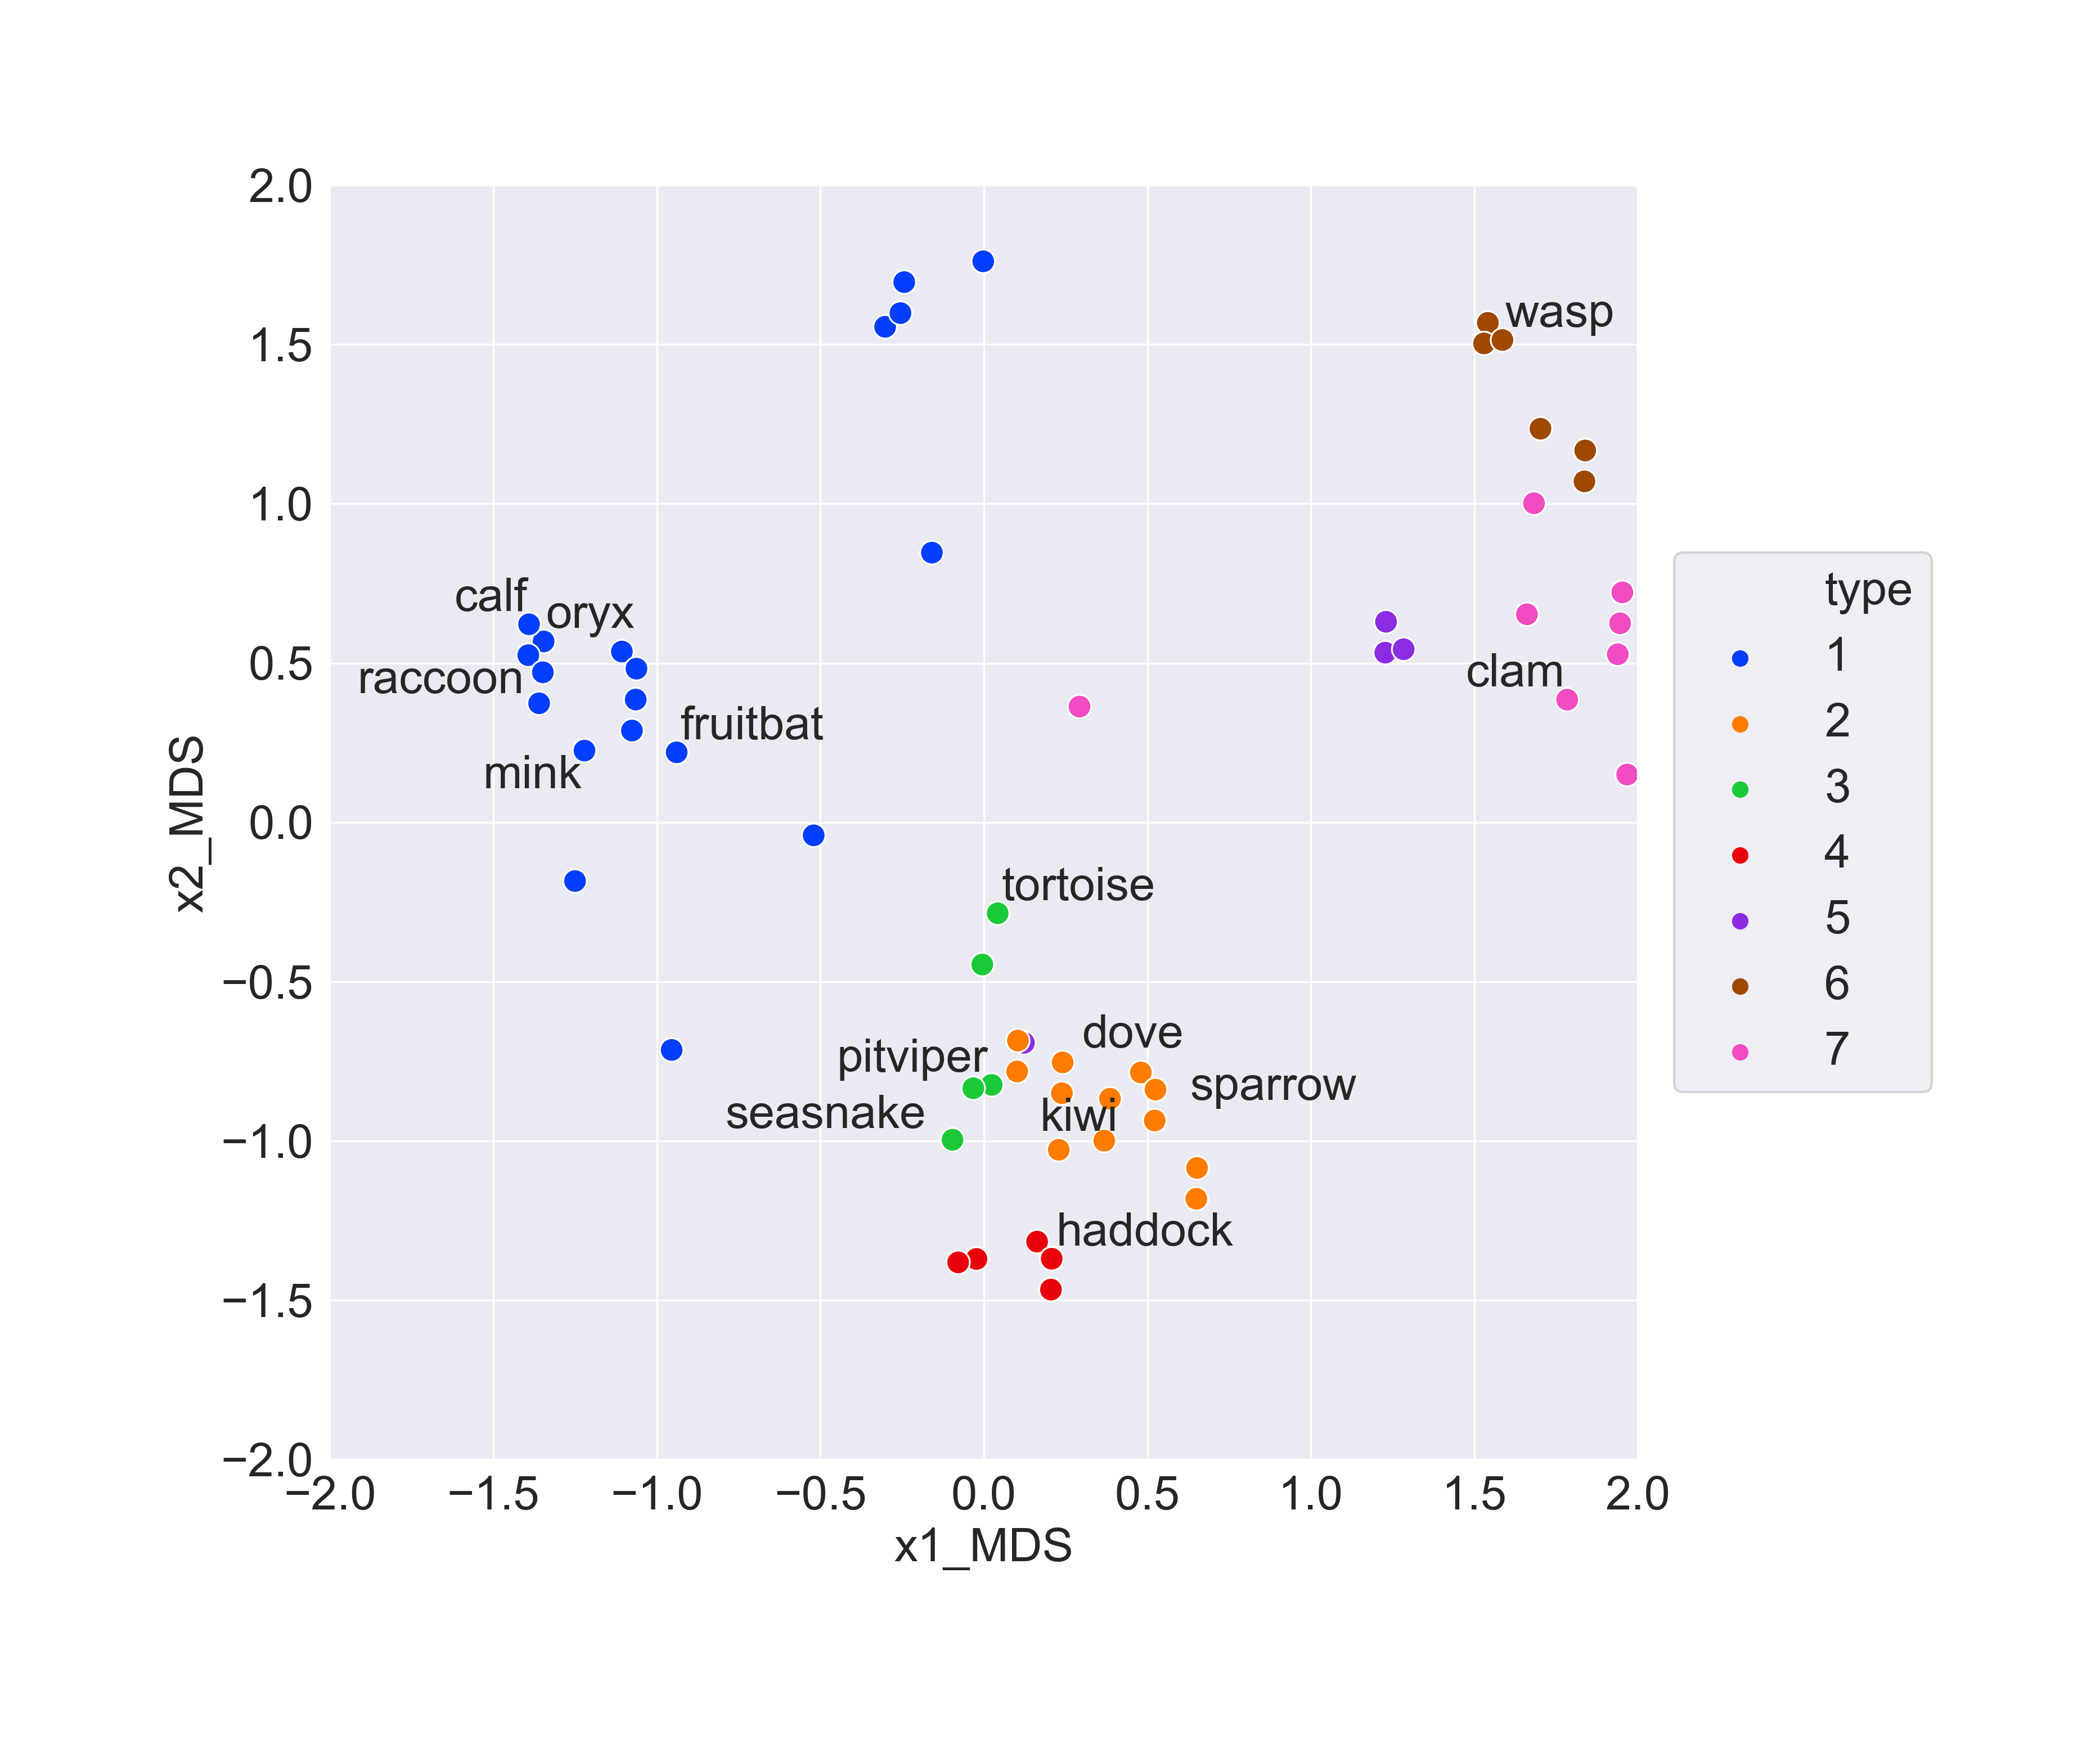
\includegraphics[width = 0.8\linewidth]{../Visualization_MDS_with_weights.png}
  \caption{Visualisation MDS, $w_{legs} = 4, w_{tail} = 4$}
  \label{vis_PCA}
\end{figure}

Here the results become a bit more interesting where I have chosen to put more weight into the number of legs an animal has and whether or not it is an aquatic animal. This has caused a clear sep


\subsection*{Isomap}
The implementation of Isomap was solved in the following manner

\begin{algorithm}[H]
\SetAlgoLined
\KwInput{Data matrix $Y$}
\KwOutput{2-dimensional embedding $X$ }
\KwData{Zoo animals}
  Select number of neighbours $k$

  Compute a graph matrix: $G \gets \text{graph\_matrix}(\text{data matrix}, k)$

  Compute shortest path matrix: $P \gets \text{shortest\_path(G)}$

  Compute similarity matrix: $S \gets \text{similarity\_matrix} (P)$

  Compute embedding: $X \gets \text{MDS}(S)$
 \caption{Isomap method}
\end{algorithm}

Argue why you should not use quadratic distance

\subsection*{Comparison}

Even though no distance in PCA, could still infer importance by scaling attributes.
